%%%%%%%%%%%%%%%%%%%%%%%%%%%%%%%%%%%%%%%%%%%%%%%%%%%%%%%%%%%%%%%%%%%
%  File name: ch3-WSt.tex
%  Title:
%  Version: 18.07.2019 (hve)
%%%%%%%%%%%%%%%%%%%%%%%%%%%%%%%%%%%%%%%%%%%%%%%%%%%%%%%%%%%%%%%%%%%
%%%%%%%%%%%%%%%%%%%%%%%%%%%%%%%%%%%%%%%%%%%%%%%%%%%%%%%%%%%%%%%%%%%
\chapter[Measures for univariate distributions]{\href{https://www.youtube.com/watch?v=ssnLQRR4kus}{Descriptive measures for univariate frequency 
distributions}}
\lb{ch3}
%%%%%%%%%%%%%%%%%%%%%%%%%%%%%%%%%%%%%%%%%%%%%%%%%%%%%%%%%%%%%%%%%%%
There are four families of scale-level-dependent standard measures 
one employs in \textbf{Statistics} to describe characteristic 
properties of univariate relative frequency distributions. On a 
technical level, the determination of the values of these measures 
from available data does not go beyond application of the four 
fundamental arithmetical operations: addition, subtraction, 
multiplication and division. We will introduce these measures in 
turn. In the following we suppose given from a \textbf{survey} for 
some one-dimensional statistical variable $X$ either (i)~a
\textbf{raw data set}~$\{x_{i}\}_{i=1,\ldots,n}$ of $n$ 
measured values, or (ii)~a \textbf{relative frequency distribution}
$(a_{j},h_{j})_{j=1,\ldots,k}$ resp.\ 
$(K_{j},h_{j})_{j=1,\ldots,k}$.

%%%%%%%%%%%%%%%%%%%%%%%%%%%%%%%%%%%%%%%%%%%%%%%%%%%%%%%%%%%%%%%%%%%
\section[Measures of central tendency]{Measures of central
tendency}
\lb{sec:lage}
%%%%%%%%%%%%%%%%%%%%%%%%%%%%%%%%%%%%%%%%%%%%%%%%%%%%%%%%%%%%%%%%%%%
Let us begin with the \textbf{measures of central tendency} which 
intend to convey a notion of ``middle'' or ``centre'' of a 
univariate relative frequency distribution.

%------------------------------------------------------------------
\subsection[Mode]{Mode}
%------------------------------------------------------------------
The \textbf{mode} $x_\mathrm{mod}$ (nom, ord, metr) of the relative 
frequency distribution for any one-dimensional variable $X$ is that 
value $a_{j}$ in $X$'s spectrum which was observed with the 
highest relative frequency in a statistical sample 
$\boldsymbol{S_{\Omega}}$. Note that the mode does not necessarily 
take a unique value.

\medskip
\noindent
\underline{\textbf{Def.:}} $h_{n}(x_\mathrm{mod}) \geq h_{n}(a_{j})$
for all $j=1,\ldots,k$.

\medskip
\noindent
\underline{EXCEL, OpenOffice:} \texttt{MODE.SNGL} (dt.:
\texttt{MODUS.EINF}, \texttt{MODALWERT}) \\
\underline{SPSS:} Analyze $\rightarrow$ Descriptive Statistics
$\rightarrow$ Frequencies \ldots $\rightarrow$ Statistics
\ldots: Mode

%------------------------------------------------------------------
\subsection[Median]{Median}
%------------------------------------------------------------------
To determine the \textbf{median} $\tilde{x}_{0.5}$ (or $Q_{2}$)
(ord, metr) of the relative frequency distribution for an ordinally
or metrically scaled one-dimensional variable $X$, it is necessary
to first arrange the $n$ observed values $\{x_{i}\}_{i=1,\ldots,n}$ 
in their ascending natural \textbf{rank order}, i.e., $x_{(1)} \leq 
x_{(2)} \leq \ldots \leq x_{(n)}$.

\medskip
\noindent
\underline{\textbf{Def.:}} For the ascendingly ordered $n$
observed values $\{x_{i}\}_{i=1,\ldots,n}$, at most 50\% have a 
rank lower or equal to resp.\ are less or equal to the median 
value $\tilde{x}_{0.5}$, and at most 50\% have a rank higher or 
equal to resp.\ are greater or equal to the median value 
$\tilde{x}_{0.5}$.

%\medskip
%\noindent
%\textbf{"`Stuhlreihenmetapher"'}: Bestimmung von Median und
% Quantilen
%
\begin{itemize}

\item[(i)] Discrete data \hfill
$\fbox{$F_{n}(\tilde{x}_{0.5})\geq 0.5$}$
%
\be
\tilde{x}_{0.5}=\begin{cases}
x_{(\frac{n+1}{2})} & \text{if}\ n\ \text{is odd} \\
\frac{1}{2}[x_{(\frac{n}{2})}+x_{(\frac{n}{2}+1)}] & \text{if}
\ n\ \text{is even}
\end{cases} \ .
\ee
%

\item[(ii)] Binned data \hfill
$\fbox{$\tilde{F}_{n}(\tilde{x}_{0.5})=0.5$}$

The class interval $K_{i}$ contains the median value 
$\tilde{x}_{0.5}$, if
$\displaystyle\sum_{j=1}^{i-1}h_{j}<0.5$ and 
$\displaystyle\sum_{j=1}^{i}h_{j}\geq 0.5$.
Then
%
\be
\tilde{x}_{0.5}=u_{i}+\frac{b_{i}}{h_{i}}
\left(0.5-\sum_{j=1}^{i-1}h_{j}\right) \ .
\ee
%
Alternatively, the median of a statistical sample 
$\boldsymbol{S_{\Omega}}$ for a continuous variable $X$ with 
binned data $(K_{j},h_{j})_{j=1,\ldots,k}$ can be obtained from 
the associated empirical cumulative distribution function by 
solving the condition 
$\tilde{F}_{n}(\tilde{x}_{0.5})\stackrel{!}{=}0.5$
for $\tilde{x}_{0.5}$; cf. Eq.~(\ref{klempvert}).\footnote{From a 
mathematical point of view, this amounts to the following problem: 
consider a straight line which contains the point with coordinates 
$(x_{0},y_{0})$ and has non-zero slope $y^{\prime}(x_{0}) \neq 0$, 
i.e., $y=y_{0}+y^{\prime}(x_{0})(x-x_{0})$. Re-arranging to solve 
for the variable $x$ then yields 
$x=x_{0}+[y^{\prime}(x_{0})]^{-1}(y-y_{0})$.}
\end{itemize}
%
\underline{\textbf{Remark:}} Note that the value of the median of a 
univariate relative frequency distribution is reasonably 
insensitive to so-called \textbf{outliers} in a statistical sample.

\medskip
\noindent
\underline{\R:} \texttt{median(\textit{variable})} \\
\underline{EXCEL, OpenOffice:} \texttt{MEDIAN}
(dt.: \texttt{MEDIAN}) \\
\underline{SPSS:} Analyze $\rightarrow$ Descriptive Statistics
$\rightarrow$ Frequencies \ldots $\rightarrow$ Statistics
\ldots: Median

%------------------------------------------------------------------
\subsection[$\alpha$--Quantile]{$\boldsymbol{\alpha}$--Quantile}
%------------------------------------------------------------------
A generalisation of the median is the concept of the
$\boldsymbol{\alpha}$\textbf{--quantile} $\tilde{x}_{\alpha}$
(ord, metr) of the relative frequency distribution for an ordinally 
or metrically scaled one-dimensional variable $X$. Again, 
it is necessary to first arrange the $n$ observed values 
$\{x_{i}\}_{i=1,\ldots,n}$ in their ascending natural \textbf{rank 
order}, i.e., $x_{(1)} \leq x_{(2)} \leq \ldots \leq x_{(n)}$.

\medskip
\noindent
\underline{\textbf{Def.:}} For the ascendingly ordered $n$
observed values $\{x_{i}\}_{i=1,\ldots,n}$, and for given $\alpha$ 
with $0<\alpha<1$, at most $\alpha\times$100\% have a rank
lower of equal to resp.\ are less or equal to the 
$\alpha$--quantile $\tilde{x}_{\alpha}$, and at most 
$(1-\alpha)\times$100\% have a rank higher or equal 
to resp.\ are greater or equal to the 
$\alpha$--quantile $\tilde{x}_{\alpha}$.
%
\begin{itemize}

\item[(i)] Discrete data \hfill
$\fbox{$F_{n}(\tilde{x}_{\alpha})\geq \alpha$}$
%
\be
\tilde{x}_{\alpha}=\begin{cases}
x_{(k)} & \text{if}\ n\alpha\notin\mathbb{N}, k>n\alpha \\
\frac{1}{2}[x_{(k)}+x_{(k+1)}] & \text{if}
\ k=n\alpha\in\mathbb{N}
\end{cases} \ .
\ee
%

\item[(ii)] Binned data \hfill
$\fbox{$\tilde{F}_{n}(\tilde{x}_{\alpha})=\alpha$}$

The class interval $K_{i}$ contains the $\alpha$--quantile 
$\tilde{x}_{\alpha}$, if
$\displaystyle\sum_{j=1}^{i-1}h_{j}<\alpha$ and 
$\displaystyle\sum_{j=1}^{i}h_{j}\geq \alpha$. Then
%
\be
\tilde{x}_{\alpha}=u_{i}+\frac{b_{i}}{h_{i}}
\left(\alpha-\sum_{j=1}^{i-1}h_{j}\right) \ .
\ee
%
Alternatively, an $\alpha$--quantile of a statistical sample 
$\boldsymbol{S_{\Omega}}$ for a continuous variable $X$ with 
binned data $(K_{j},h_{j})_{j=1,\ldots,k}$ can be obtained from 
the associated empirical cumulative distribution function by 
solving the condition 
$\tilde{F}_{n}(\tilde{x}_{\alpha})\stackrel{!}{=}\alpha$
for $\tilde{x}_{\alpha}$; cf. Eq.~(\ref{klempvert}).
%\textbf{"`Hochsprungmetapher"'}: Bestimmung von $\tilde{x}_{\alpha}$

\end{itemize}
%
\underline{\textbf{Remark:}} The quantiles
$\tilde{x}_{0.25}$, $\tilde{x}_{0.5}$, $\tilde{x}_{0.75}$
(also denoted by $Q_{1}$, $Q_{2}$, $Q_{3}$) have special status. 
They are referred to as the \textbf{first quartile} $\rightarrow$
\textbf{second quartile (median)} $\rightarrow$
\textbf{third quartile} of a relative frequency distribution for an 
ordinally or a metrically scaled one-dimensional variable $X$ and 
form the core of the \textbf{five number summary} of this 
distribution. Occasionally, $\alpha$--quantiles are also referred 
to as \textbf{percentile values}.

\medskip
\noindent
\underline{\R:} \texttt{quantile(\textit{variable}, $\alpha$)} \\
\underline{EXCEL, OpenOffice:} \texttt{PERCENTILE.EXC}
(dt.: \texttt{QUANTIL.EXKL}, \texttt{QUANTIL}) \\
\underline{SPSS:} Analyze $\rightarrow$ Descriptive Statistics
$\rightarrow$ Frequencies \ldots $\rightarrow$ Statistics
\ldots: Percentile(s)

%------------------------------------------------------------------
\subsection[Five number summary]{Five number summary}
%------------------------------------------------------------------
The \textbf{five number summary} (ord, metr) of the relative 
frequency distribution for an ordinally or metrically scaled 
one-dimensional variable $X$ is a compact compilation of 
information giving the (i)~lowest rank resp.\ smallest value, 
(ii)~first quartile, (iii)~second quartile or median, (iv)~third 
quartile, and (v)~highest rank resp.\ largest value that $X$ takes 
in a univariate raw data set $\{x_{i}\}_{i=1,\ldots,n}$ from a 
statistical sample $\boldsymbol{S_{\Omega}}$, i.e.,
%
\be
\{x_{(1)}, \tilde{x}_{0.25}, \tilde{x}_{0.5},
\tilde{x}_{0.75}, x_{(n)}\} \ .
\ee
%
Alternative notation: $\{Q_{0}, Q_{1}, Q_{2}, Q_{3}, Q_{4}\}$.

\medskip
\noindent
\underline{\R:} \texttt{fivenum(\textit{variable})},
\texttt{summary(\textit{variable})} \\
\underline{EXCEL, OpenOffice:} \texttt{MIN}, \texttt{QUARTILE.INC},
\texttt{MAX} (dt.: \texttt{MIN}, \texttt{QUARTILE.INKL},
\texttt{QUARTILE}, \texttt{MAX})\\
\underline{SPSS:} Analyze $\rightarrow$ Descriptive Statistics
$\rightarrow$ Frequencies \ldots $\rightarrow$ Statistics
\ldots: Quartiles, Minimum, Maximum

\medskip
\noindent
All measures of central tendency which we will discuss hereafter 
are defined exclusively for characterising relative frequency 
distributions for \textit{metrically scaled one-dimensional 
variables}~$X$ only.

%------------------------------------------------------------------
\subsection[Sample mean]{Sample mean}
%------------------------------------------------------------------
The best known measure of central tendency is the dimensionful
\textbf{sample mean} $\bar{x}$ (metr) (also referred to as the 
arithmetical mean). Amongst the first to have employed the sample 
mean as a characteristic statistical measure in the systematic 
analysis of quantitative emprical data ranks the English 
physicist, mathematician, astronomer and philosopher
\href{http://www-history.mcs.st-and.ac.uk/Biographies/Newton.html}{Sir
Isaac Newton PRS MP (1643--1727)}; cf. Mlodinow 
(2008)~\ct[p~127]{mlo2008}. Given metrically scaled data, it is 
defined by:
%
\begin{itemize}
\item[(i)] From a raw data set:
%
\be
\lb{eq:arithmean1}
\fbox{$\displaystyle
\bar{x}
:= \frac{1}{n}\left(x_{1}+\ldots+x_{n}\right)
=: \frac{1}{n}\sum_{i=1}^{n}x_{i} \ .
$}
\ee
%
\item[(ii)] From a relative frequency distribution:
%
\be
\bar{x}
\lb{eq:arithmean2}
:= a_{1}h_{n}(a_{1})+\ldots+a_{k}h_{n}(a_{k})
=: \sum_{j=1}^{k}a_{j}h_{n}(a_{j}) \ .
\ee
%
\end{itemize}
%

\medskip
\noindent
\underline{\textbf{Remarks:}} (i)~The value of the sample mean is
very sensitive to \textbf{outliers}.\\ (ii)~For binned data one
selects the midpoint of each class interval $K_{i}$ to represent
the $a_{j}$ (provided the raw data set is no longer accessible).

\medskip
\noindent
\underline{\R:} \texttt{mean(\textit{variable})} \\
\underline{EXCEL, OpenOffice:} \texttt{AVERAGE} (dt.:
\texttt{MITTELWERT}) \\
\underline{SPSS:} Analyze $\rightarrow$ Descriptive Statistics
$\rightarrow$ Frequencies \ldots $\rightarrow$ Statistics
\ldots: Mean


%------------------------------------------------------------------
\subsection[Weighted mean]{Weighted mean}
%------------------------------------------------------------------
In practice, one also encounters the dimensionful \textbf{weighted 
mean} $\bar{x}_{w}$ (metr), defined by
%
\be
\fbox{$\displaystyle
\bar{x}_{w}
:= w_{1}x_{1}+\ldots+w_{n}x_{n}
=: \sum_{i=1}^{n}w_{i}x_{i} \ ;
$}
\ee
%
the $n$ \textbf{weight factors} $w_{1}$, \ldots, $w_{n}$ need to 
satisfy the constraints
%
\be
0 \leq w_{1}, \ldots, w_{n} \leq 1
\quad \text{and} \quad
w_{1}+\ldots+w_{n}=\sum_{i=1}^{n}w_{i}=1 \ .
\ee
%

%%%%%%%%%%%%%%%%%%%%%%%%%%%%%%%%%%%%%%%%%%%%%%%%%%%%%%%%%%%%%%%%%%%
\section[Measures of variability]{Measures of variability}
\lb{sec:streuung}
%%%%%%%%%%%%%%%%%%%%%%%%%%%%%%%%%%%%%%%%%%%%%%%%%%%%%%%%%%%%%%%%%%%
The idea behind the \textbf{measures of variability} is to convey a 
notion of the ``spread'' of data in a given statistical sample 
$\boldsymbol{S_{\Omega}}$, technically referred to also as the 
\textbf{dispersion} of the data. As the realisation of this
intention requires a well-defined concept of \textbf{distance}, 
the measures of variability are meaningful for data relating to 
\textit{metrically scaled one-dimensional variables}~$X$ only. One 
can distinguish two kinds of such measures: (i)~simple 
$2$-data-point measures, and (ii)~sophisticated $n$-data-point 
measures. We begin with two examples belonging to the first 
category.

%------------------------------------------------------------------
\subsection[Range]{Range}
%------------------------------------------------------------------
For a univariate raw data set $\{x_{i}\}_{i=1,\ldots,n}$ of $n$ 
observed values for $X$, the dimensionful \textbf{range} $R$ (metr) 
simply expresses the difference between the largest and the 
smallest value in this set, i.e.,
%
\be
\lb{eq:range}
R:=x_{(n)}-x_{(1)} \ .
\ee
%
The basis of this measure is the ascendingly ordered data set 
$x_{(1)} \leq x_{(2)} \leq \ldots \leq x_{(n)}$. Alternatively, 
the range can be denoted by $R=Q_{4}-Q_{0}$.

\medskip
\noindent
\underline{\R:} \texttt{range(\textit{variable})},
$\texttt{max(\textit{variable})}
- \texttt{min(\textit{variable})}$ \\
\underline{SPSS:} Analyze $\rightarrow$ Descriptive Statistics
$\rightarrow$ Frequencies \ldots $\rightarrow$ Statistics
\ldots: Range

%------------------------------------------------------------------
\subsection[Interquartile range]{Interquartile range}
%------------------------------------------------------------------
In the same spirit as the range, the dimensionful
\textbf{interquartile range} $d_{Q}$ (metr) is defined as the 
difference between the third quantile and the first quantile of 
the relative frequency distribution for some metrically scaled
$X$, i.e.,
%
\be
d_{Q}:=\tilde{x}_{0.75}-\tilde{x}_{0.25} \ .
\ee
%
Alternatively, this is $d_{Q}=Q_{3}-Q_{1}$.

\medskip
\noindent
\underline{\R:} \texttt{IQR(\textit{variable})}

\medskip
\noindent
Viewing the interquartile range~$d_{Q}$ of a univariate metrically
scaled raw data set~$\{x_{i}\}_{i=1,\ldots,n}$ as a reference
length, it is commonplace to define a specific value~$x_{i}$ to be
an
%
\begin{itemize}

\item \textbf{outlier}, if either $x_{i} < \tilde{x}_{0.25}
- 1.5d_{Q}$ and $x_{i} \geq \tilde{x}_{0.25}
- 3d_{Q}$, or $x_{i} > \tilde{x}_{0.75} + 1.5d_{Q}$ and
$x_{i} \leq \tilde{x}_{0.75} + 3d_{Q}$,

\item \textbf{extreme value}, if either $x_{i} < \tilde{x}_{0.25}
- 3d_{Q}$, or $x_{i} > \tilde{x}_{0.75} + 3d_{Q}$.

\end{itemize}
%

\medskip
\noindent
A very convenient graphical method for transparently displaying 
distributional features of metrically scaled data relating to a 
five number summary, also making explicit the interquartile
range, outliers and extreme values, is provided by a \textbf{box
plot}; see, e.g., Tukey (1977)~\ct{tuk1977}. An example of a single
box plot is depicted in Fig.~\ref{fig:1Dboxplot}, of parallel
box plots in Fig.~\ref{fig:parallelBoxplots}.

\medskip
\noindent
\underline{\R:} \texttt{boxplot(\textit{variable})},
\texttt{boxplot(\textit{variable}~\texttildelow~\textit{group
variable})}

%
\begin{figure}[!htb]
\begin{center}
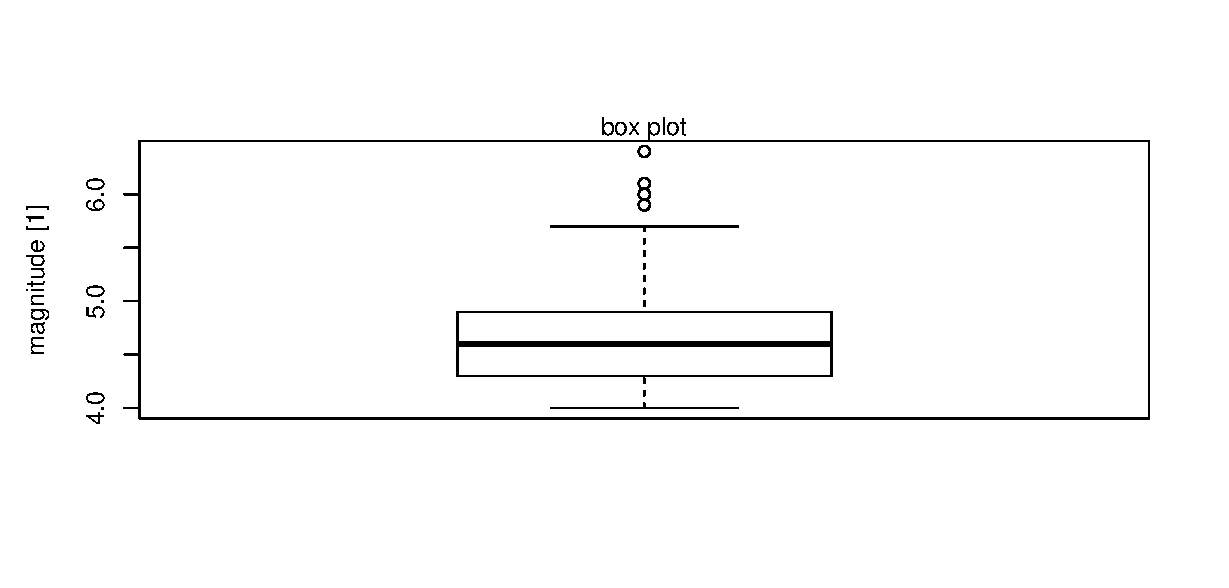
\includegraphics[scale=0.8]{1Dboxplot.eps}
\end{center}
\caption{Example of a box plot, representing elements of the five
number summary for the distribution of measured values for the
variable ``magnitude'' in the \R{} data set ``quakes.'' The open
circles indicate the positions of outliers. \newline
\underline{\R:} \newline
\texttt{data("quakes")} \newline
\texttt{?quakes} \newline
\texttt{boxplot( quakes\$mag )}}
\lb{fig:1Dboxplot}
\end{figure}
%

%
\begin{figure}[!htb]
\begin{center}
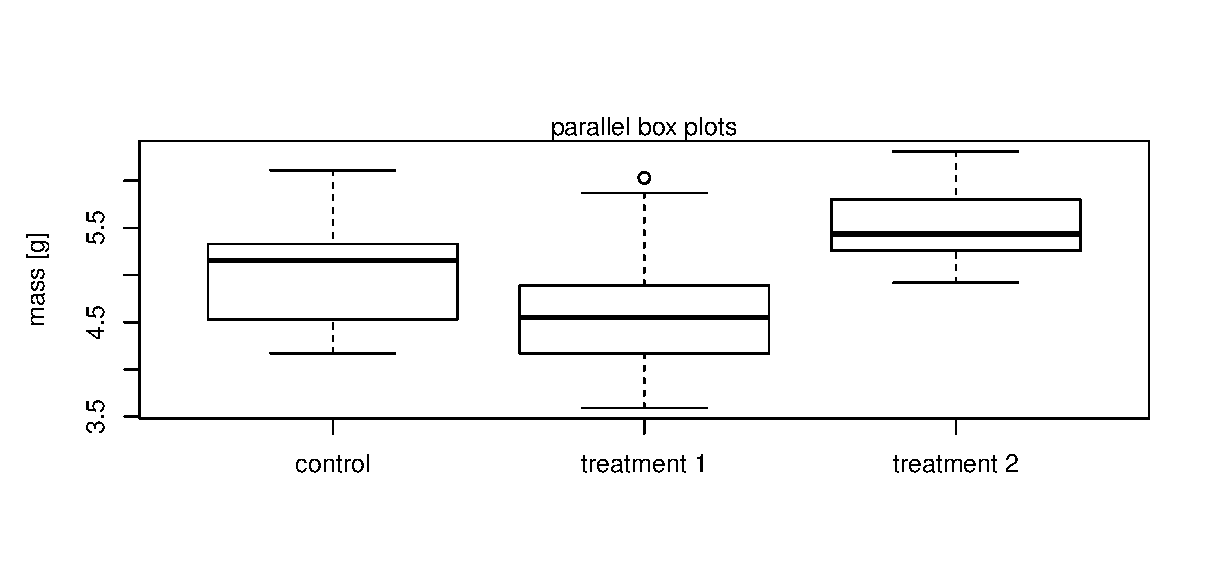
\includegraphics[scale=0.8]{parallelBoxplots.eps}
\end{center}
\caption{Example of parallel box plots, comparing elements of
the five number summary for the distribution of measured values for
the variable ``weight'' between categories of the variable
``group'' in the \R{} data set ``PlantGrowth.'' The open
circle indicates the position of an outlier. \newline
\underline{\R:} \newline
\texttt{data("PlantGrowth")} \newline
\texttt{?PlantGrowth} \newline
\texttt{boxplot( PlantGrowth\$weight~\texttildelow~PlantGrowth\$group )}}
\lb{fig:parallelBoxplots}
\end{figure}
%

%%------------------------------------------------------------------
%\subsection[Mean absolute deviation from median]{Mean absolute
%deviation from median}
%%------------------------------------------------------------------
%\textbf{mean absolute deviation from the median} $\tilde{d}_{0.5}$
%
%\begin{itemize}
%
%\item[(i)] From raw data set:
%%
%\be
%\tilde{d}_{0.5}:=\frac{1}{n}\sum_{i=1}^{n}
%\left|x_{i}-\tilde{x}_{0.5}\right|
%\ee
%%
%\item[(ii)] From relative frequency distribution:
%%
%\be
%\tilde{d}_{0.5}:= \sum_{j=1}^{k}
%\left|a_{j}-\tilde{x}_{0.5}\right|h_{n}(a_{j})
%\ee
%%
%
%\end{itemize}

%------------------------------------------------------------------
\subsection[Sample variance]{Sample variance}
%------------------------------------------------------------------
The most frequently employed measure of variability in \textbf{
Statistics} is the dimensionful $n$-data-point \textbf{sample 
variance} $s^{2}$ (metr), and the related sample standard 
deviation to be discussed below. One of the originators of these 
concepts is the French mathematician 
\href{http://www-history.mcs.st-and.ac.uk/Biographies/De_Moivre.html}{Abraham de Moivre (1667--1754)}; cf. Bernstein (1998)~\ct[p~5]{ber1998}.
Given a univariate raw data set  
$\{x_{i}\}_{i=1,\ldots,n}$ for $X$, its spread is essentially 
quantified in terms of the sum of squared deviations of the $n$ 
data points~$x_{i}$ from their common sample mean~$\bar{x}$. Due 
to the algebraic identity
%
\[
\left(x_{1}-\bar{x}\right) + \ldots + \left(x_{n}-\bar{x}\right)
= \sum_{i=1}^{n}\left(x_{i}-\bar{x}\right)
= \left(\sum_{i=1}^{n}x_{i}\right) - n\bar{x}
\stackrel{\text{Eq.}~(\ref{eq:arithmean1})}{\equiv} 0 \ ,
\]
%
there are only $n-1$ \textbf{degrees of freedom} involved in this 
measure. The sample variance is thus defined by:
%
\begin{itemize}
\item[(i)] From a raw data set:
%
\be
\lb{eq:sampvardescr}
\fbox{$\displaystyle
s^{2} := 
\frac{1}{n-1}\left[\,(x_{1}-\bar{x})^{2}+\ldots+(x_{n}-\bar{x})^{2}
\,\right]
=: \frac{1}{n-1}\sum_{i=1}^{n}\left(x_{i}-\bar{x}\right)^{2} \ ;
$}
\ee
%
alternatively, by the \textbf{shift theorem}:\footnote{That is,
the algebraic identity 
$\displaystyle\sum_{i=1}^{n}\left(x_{i}-\bar{x}\right)^{2}
= \sum_{i=1}^{n}\left(x_{i}^{2}-2x_{i}\bar{x}+\bar{x}^{2}\right)
\stackrel{\text{Eq.}~(\ref{eq:arithmean1})}{\equiv} 
\sum_{i=1}^{n}x_{i}^{2}-\sum_{i=1}^{n}\bar{x}^{2}
= \sum_{i=1}^{n}x_{i}^{2}-n\bar{x}^{2}$.}
%
\be
\lb{eq:sampvardescr2}
s^{2}
= \frac{1}{n-1}\left[\,x_{1}^{2}+\ldots+x_{n}^{2}-n\bar{x}{}^{2}
\,\right]
= \frac{1}{n-1}\left[\,\sum_{i=1}^{n}x_{i}^{2}-n\bar{x}{}^{2}
\,\right] \ .
\ee
%
\item[(ii)] From a relative frequency distribution:
%
\begin{eqnarray}
\lb{eq:ssqurel1}
s^{2}
& := & \frac{n}{n-1}\left[\,(a_{1}-\bar{x})^{2}h_{n}(a_{1})+\ldots
+(a_{k}-\bar{x})^{2}h_{n}(a_{k})\,\right] \nonumber\\
& =: & \frac{n}{n-1}\sum_{j=1}^{k}\left(a_{j}-\bar{x}\right)^{2}
h_{n}(a_{j}) \ ;
\end{eqnarray}
%
alternatively:
%
\begin{eqnarray}
\lb{eq:ssqurel2}
s^{2}
& = & \frac{n}{n-1}\left[\,a_{1}^{2}h_{n}(a_{1})+\ldots
+a_{k}^{2}h_{n}(a_{k})-\bar{x}{}^{2}\,\right] \nonumber\\
& = & \frac{n}{n-1}\left[\,\sum_{j=1}^{k}a_{j}^{2}h_{n}(a_{j})
-\bar{x}{}^{2}\,\right] \ .
\end{eqnarray}
%

\end{itemize}
%
\underline{\textbf{Remarks:}} (i)~We point out that the alternative 
formulae for a sample variance provided here prove computationally 
more efficient.\\
(ii)~For binned data, when one selects the midpoint of each class 
interval $K_{j}$ to represent the~$a_{j}$ (given the raw data set 
is no longer accessible), a correction of Eqs.~(\ref{eq:ssqurel1}) 
and (\ref{eq:ssqurel2}) by an additional term 
$(1/12)(n/n-1)\sum_{j=1}^{k}b_{j}^{2}h_{j}$ becomes necessary,
assuming uniformly distributed data within each of the class
intervals $K_{j}$ of width $b_{j}$; cf. Eq.~(\ref{eq:varUniDistr}).

\medskip
\noindent
\underline{\R:} \texttt{var(\textit{variable})} \\
\underline{EXCEL, OpenOffice:} \texttt{VAR.S} (dt.: \texttt{VAR.S},
\texttt{VARIANZ}) \\
\underline{SPSS:} Analyze $\rightarrow$ Descriptive Statistics
$\rightarrow$ Frequencies \ldots $\rightarrow$ Statistics
\ldots: Variance

%------------------------------------------------------------------
\subsection[Sample standard deviation]{Sample standard deviation}
%------------------------------------------------------------------
For ease of handling dimensions associated with a metrically 
scaled one-dimensional variable $X$, one defines the dimensionful 
\textbf{sample standard deviation} $s$ (metr) simply as the positive 
square root of the sample variance~(\ref{eq:sampvardescr}), i.e.,
%
\be
s := +\sqrt{s^{2}} \ ,
\ee
%
such that a measure for the spread of data results which shares 
the dimension of $X$ and its sample mean~$\bar{x}$.

\medskip
\noindent
\underline{\R:} \texttt{sd(\textit{variable})} \\
\underline{EXCEL, OpenOffice:} \texttt{STDEV.S} (dt.:
\texttt{STABW.S}, \texttt{STABW}) \\
\underline{SPSS:} Analyze $\rightarrow$ Descriptive Statistics
$\rightarrow$ Frequencies \ldots $\rightarrow$ Statistics
\ldots: Std. deviation

%------------------------------------------------------------------
\subsection[Sample coefficient of variation]{Sample coefficient of
variation}
%------------------------------------------------------------------
For ratio scaled one-dimensional variables $X$, a dimensionless 
relative measure of variability is the \textbf{sample coefficient of 
variation} $v$ (metr: ratio), defined by
%
\be
v := \frac{s}{\bar{x}} \ ,
\quad\text{if}\quad
\bar{x} > 0 \ .
\ee
%

%------------------------------------------------------------------
\subsection[Standardisation]{Standardisation}
%------------------------------------------------------------------
Data for metrically scaled one-dimensional variables $X$ is 
amenable to the process of \textbf{standardisation}. By this is meant 
a linear affine transformation~$X \rightarrow Z$, which generates 
from a univariate raw data set $\{x_{i}\}_{i=1,\ldots,n}$ of $n$ 
measured values for a dimensionful variable $X$, with sample mean 
$\bar{x}$ and sample standard deviation $s_{X}>0$, data for an 
equivalent dimensionless variable $Z$ according to
%
\be
\lb{eq:standardisationdiscriptive}
\fbox{$\displaystyle
x_{i} \mapsto z_{i}:=\frac{x_{i}-\bar{x}}{s_{X}}
\qquad \text{for all}\ i=1,\ldots,n \ .
$}
\ee
%
For the resultant $Z$-data, referred to as the
\textbf{$\boldsymbol{Z}$ scores} of the original metrical $X$-data,
this has the convenient practical consequences that (i)~all 
one-dimensional metrical data is thus represented on the 
\textit{same dimensionless measurement scale}, and
(ii)~the corresponding sample mean and sample standard deviation of
the $Z$-data amount to
%
\[
\bar{z} = 0
\quad\text{and}\quad s_{Z}=1 \ ,
\]
%
respectively. Employing Z scores, specific values~$x_{i}$ of the
original metrical $X$-data will be expressed in terms of sample
standard deviation units, i.e., by how many sample standard
deviations they fall on either side of the common sample mean.
Essential information on characteristic distributional features of
one-dimensional metrical data will be preserved by the process of standardisation.

\medskip
\noindent
\underline{\R:} \texttt{scale(\textit{variable}, center = TRUE,
scale = TRUE)} \\
\underline{EXCEL, OpenOffice:} \texttt{STANDARDIZE} (dt.:
\texttt{STANDARDISIERUNG})\\
\underline{SPSS:} Analyze $\rightarrow$ Descriptive Statistics
$\rightarrow$ Descriptives \ldots $\rightarrow$ Save standardized 
values as variables

%%%%%%%%%%%%%%%%%%%%%%%%%%%%%%%%%%%%%%%%%%%%%%%%%%%%%%%%%%%%%%%%%%%
\section[Measures of relative distortion]{Measures of relative
distortion}
\lb{sec:distortion}
%%%%%%%%%%%%%%%%%%%%%%%%%%%%%%%%%%%%%%%%%%%%%%%%%%%%%%%%%%%%%%%%%%%
The third family of measures characterising relative frequency 
distributions for univariate data~$\{x_{i}\}_{i=1,\ldots,n}$ for 
metrically scaled one-dimensional variables~$X$, having specific 
sample mean~$\bar{x}$ and sample standard deviation~$s_{X}$, 
relate to the issue of the \textbf{shape} of a distribution. These 
measures take a \textbf{Gau\ss ian normal distribution} (cf. 
Sec.~\ref{sec:normverteil} below) as as a reference case, with the
values of its two free parameters equal to the given $\bar{x}$
and~$s_{X}$. With respect to this \textit{reference distribution},
one defines two kinds of dimensionless \textbf{measures of relative
distortion} as described in the following (cf., e.g., Joanes and
Gill (1998)~\ct{joagil1998}).

%------------------------------------------------------------------
\subsection[Skewness]{Skewness}
\lb{subsec:skew}
%------------------------------------------------------------------
The \textbf{skewness} $g_{1}$ (metr) is a dimensionless measure to 
quantify the degree of relative distortion of a given frequency
distribution in the \textit{horizontal direction}. Its 
implementation in the software package EXCEL employs the definition
%
\be
\lb{eq:scew}
g_{1} := 
\frac{n}{(n-1)(n-2)}\sum_{i=1}^{n}\left(\frac{x_{i}-\bar{x}}{s_{X}}
\right)^{3}
\qquad\text{for}\quad n > 2 \ ,
\ee
%
wherein the observed values $\{x_{i}\}_{i=1,\ldots,n}$ enter in 
their standardised form according to 
Eq.~(\ref{eq:standardisationdiscriptive}). Note that $g_{1}=0$ for 
an exact Gau\ss ian normal distribution.

\medskip
\noindent
\underline{\R:} \texttt{skewness(\textit{variable},
type = 2)} (package: \texttt{e1071}, by Meyer \textit{et al}
(2019)~\ct{meyetal2019}) \\
\underline{EXCEL, OpenOffice:} \texttt{SKEW} (dt.:
\texttt{SCHIEFE}) \\
\underline{SPSS:} Analyze $\rightarrow$ Descriptive Statistics
$\rightarrow$ Frequencies \ldots $\rightarrow$ Statistics
\ldots: Skewness

%------------------------------------------------------------------
\subsection[Excess kurtosis]{Excess kurtosis}
\lb{subsec:kurt}
%------------------------------------------------------------------
The \textbf{excess kurtosis} $g_{2}$ (metr) is a dimensionless 
measure to quantify the degree of relative distortion of a given 
frequency distribution in the \textit{vertical direction}. Its 
implementation in the software package EXCEL employs the definition
%
\be
\lb{eq:kurt}
g_{2} := 
\frac{n(n+1)}{(n-1)(n-2)(n-3)}\sum_{i=1}^{n}\left(\frac{x_{i}
-\bar{x}}{s_{X}}\right)^{4} - \frac{3(n-1)^{2}}{(n-2)(n-3)}
\qquad\text{for}\quad n > 3 \ ,
\ee
%
wherein the observed values $\{x_{i}\}_{i=1,\ldots,n}$ enter in
their standardised form according to 
Eq.~(\ref{eq:standardisationdiscriptive}). Note that $g_{2}=0$ for 
an exact Gau\ss ian normal distribution.

\medskip
\noindent
\underline{\R:} \texttt{kurtosis(\textit{variable},
type = 2)} (package: \texttt{e1071}, by Meyer \textit{et al}
(2019)~\ct{meyetal2019}) \\
\underline{EXCEL, OpenOffice:} \texttt{KURT} (dt.:
\texttt{KURT}) \\
\underline{SPSS:} Analyze $\rightarrow$ Descriptive Statistics
$\rightarrow$ Frequencies \ldots $\rightarrow$ Statistics
\ldots: Kurtosis

%%%%%%%%%%%%%%%%%%%%%%%%%%%%%%%%%%%%%%%%%%%%%%%%%%%%%%%%%%%%%%%%%%%
\section[Measures of concentration]{Measures of concentration}
\lb{sec:konz}
%%%%%%%%%%%%%%%%%%%%%%%%%%%%%%%%%%%%%%%%%%%%%%%%%%%%%%%%%%%%%%%%%%%
Finally, for univariate data~$\{x_{i}\}_{i=1,\ldots,n}$ relating 
to a ratio scaled one-dimensional variable $X$, which has a 
discrete spectrum of values $\{a_{j}\}_{j=1,\ldots,k}$, or which
was binned into $k$~different categories $\{K_{j}\}_{j=1,\ldots,k}$ 
with respective midpoints $a_{j}$, two kinds of \textbf{measures of 
concentration} are commonplace in \textbf{Statistics}; one 
qualitative in nature, the other quantitative.


\medskip
\noindent
Begin by defining the \textbf{total sum} for the data 
$\{x_{i}\}_{i=1,\ldots,n}$ by
%
\be
\lb{eq:totalsum}
S := \sum_{i=1}^{n}x_{i}
= \sum_{j=1}^{k}a_{j}o_{n}(a_{j})
\stackrel{\text{Eq.}~(\ref{eq:arithmean1})}{=} n\bar{x} \ ,
\ee
%
where $(a_{j},o_{n}(a_{j}))_{j=1,\ldots,k}$ is the absolute 
frequency distribution for the observed values (or categories) 
of~$X$. Then the \textbf{relative proportion} that the value
$a_{j}$ (or the category $K_{j}$) takes in~$S$ is
%
\be
\lb{eq:relprop}
\frac{a_{j}o_{n}(a_{j})}{S} = \frac{a_{j}h_{n}(a_{j})}{\bar{x}} \ .
\ee
%

%------------------------------------------------------------------
\subsection[Lorenz curve]{Lorenz curve}
\lb{subsec:lorenz}
%------------------------------------------------------------------
From the elements introduced in Eqs.~(\ref{eq:totalsum}) and 
(\ref{eq:relprop}), the US--American economist
\href{http://en.wikipedia.org/wiki/Max_O._Lorenz}{Max Otto Lorenz 
(1876--1959)} constructed cumulative relative quantities which 
constitute the coordinates of a so-called \textbf{Lorenz curve} 
representing concentration in the %relative frequency
distribution for the ratio scaled one-dimensional variable $X$; cf. 
Lorenz (1905)~\ct{lor1905}. These coordinates are defined as 
follows:
%
\begin{itemize}
\item Horizontal axis:
%
\be
k_{i} := \sum_{j=1}^{i}\frac{o_{n}(a_{j})}{n}
= \sum_{j=1}^{i}h_{n}(a_{j})
\qquad (i=1,\ldots,k) \ ,
\ee
%
\item Vertical axis:
%
\be
l_{i} := \sum_{j=1}^{i}\frac{a_{j}o_{n}(a_{j})}{S}
= \sum_{j=1}^{i}\frac{a_{j}h_{n}(a_{j})}{\bar{x}}
\qquad (i=1,\ldots,k) \ .
\ee
%
\end{itemize}
%
The initial point on a Lorenz curve is generally the coordinate
system's origin, $(k_{0},l_{0})=(0,0)$, the final point 
is $(1,1)$. As a reference facility to measure concentration in 
the distribution of $X$ in qualitative terms, one defines a
\textbf{null concentration curve} as the bisecting line linking
$(0,0)$ to $(1,1)$. The Lorenz curve is interpreted as stating that
a point on the curve with coordinates $(k_{i},l_{i})$ represents
the fact that $k_{i}\times 100\%$ of the $n$ statistical units take
a share of $l_{i}\times 100\%$ in the total sum $S$ for the ratio
scaled one-dimensional variable $X$. Qualitatively, for given
univariate data~$\{x_{i}\}_{i=1,\ldots,n}$, the concentration in
the distribution of $X$ is the stronger, the larger is the dip of
the Lorenz curve relative to the null concentration curve. Note
that in addition to the null concentration curve, one can define as
a second reference facility a \textbf{maximum concentration curve}
such that only the largest value $a_{k}$ (or category $K_{k}$) in
the spectrum of values of $X$ takes the full share of $100\%$ in
the total sum $S$ for $\{x_{i}\}_{i=1,\ldots,n}$.

%------------------------------------------------------------------
\subsection[Normalised Gini coefficient]{Normalised Gini 
coefficient}
\lb{subsec:gini}
%------------------------------------------------------------------
The Italian statistician, demographer and sociologist
\href{http://en.wikipedia.org/wiki/Corrado_Gini}{Corrado
Gini (1884--1965)} devised a quantitative measure for 
concentration in the distribution for a ratio scaled
one-dimensional variable~$X$; cf. Gini (1921)~\ct{gin1921}. The
dimensionless \textbf{normalised Gini coefficient} $G_{+}$ (metr:
ratio) can be interpreted geometrically as the ratio of areas
%
\be
G_{+} := \frac{(\text{area enclosed between Lorenz and
null concentration curves})}{(\text{area enclosed between maximum 
and null concentration curves})} \ .
\ee
%
Its related computational definition is given by
%
\be
\fbox{$\displaystyle
G_{+} := \frac{n}{n-1}\left[\,\sum_{i=1}^{k}(k_{i-1}+k_{i})\,
\frac{a_{i}o_{n}(a_{i})}{S}-1\,\right] \ .
$}
\ee
%
Due to normalisation, the range of values is $0 \leq G_{+} \leq 1$.
Thus, null concentration amounts to $G_{+}=0$, while maximum 
concentration amounts to $G_{+}=1$.\footnote{In September 2012 it 
was reported (implicitly) in the public press that the coordinates 
underlying the Lorenz curve describing the distribution of private 
equity in Germany at the time were $(0.00,0.00)$, $(0.50,0.01)$, 
$(0.90,0.50)$, and $(1.00,1.00)$; cf. Ref.~\ct{sue2012}. Given 
that in this case $n \gg 1$, these values amount to a Gini 
coefficient of $G_{+}=0.64$. The Oxfam Report on Wealth Inequality
2019 can be found at the URL (cited on May 31, 2019):
\href{https://www.oxfam.org/en/research/public-good-or-private-wealth}{www.oxfam.org/en/research/public-good-or-private-wealth}.}

%%%%%%%%%%%%%%%%%%%%%%%%%%%%%%%%%%%%%%%%%%%%%%%%%%%%%%%%%%%%%%%%%%%
%%%%%%%%%%%%%%%%%%%%%%%%%%%%%%%%%%%%%%%%%%%%%%%%%%%%%%%%%%%%%%%%%%%
